\documentclass[tikz,border=10pt]{standalone}
\begin{document}
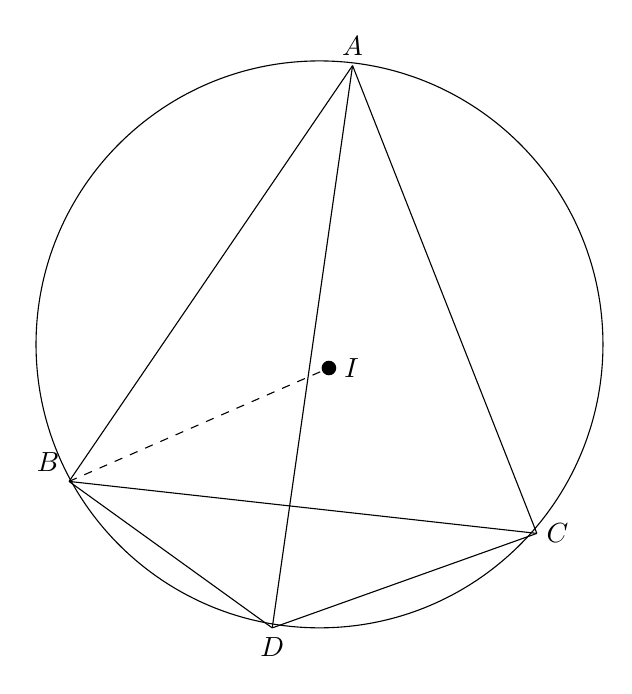
\begin{tikzpicture}[scale=1.2]
  % circle
  \draw (0,0) circle (3);
  % points
  \coordinate (A) at (0.35,2.95);
  \coordinate (B) at (-2.65,-1.45);
  \coordinate (C) at (2.3,-2.0);
  \coordinate (D) at (-0.5,-3.0);
  \coordinate (I) at (0.1,-0.25);
  % edges
  \draw (A) -- (B);
  \draw (A) -- (C);
  \draw (B) -- (C);
  \draw (A) -- (D);
  \draw (B) -- (D);
  \draw (C) -- (D);
  \draw[dashed] (B) -- (I);
  % point I
  \fill (I) circle (2.2pt);
  % labels
  \node[above] at (A) {$A$};
  \node[above left] at (B) {$B$};
  \node[right] at (C) {$C$};
  \node[below] at (D) {$D$};
  \node[right=2pt] at (I) {$I$};
\end{tikzpicture}
\end{document}
